\documentclass[a4paper,12pt]{article}
\usepackage[utf8]{inputenc}
\usepackage{amsmath,amsfonts,tikz,hyperref}
\usepackage{fontenc}
\usepackage{graphicx}
\usepackage[euler-digits]{eulervm}
\title{FinElt Quick Start Guide}
\author{William McLean}
\date{\today}
%%%%%%%%%%%%%%%%%%%%%%%%%%%%%%%%%%%%%%%%%%%%%%%%%%%%%%%%%%%%%%%%%%%%%%
\begin{document}
\maketitle
To use FinElt you need to install \href{www.julialan.org}{Julia}~and 
\href{www.geuz.org/gmsh/}{Gmsh}~\cite{Gmsh}.  Versions for Windows or 
OS~X can be downloaded from the project websites.  Under Linux, you
might be able to use your distribution's package manager.  For 
example, I develop FinElt on \href{www.fedoraproject.org}{Fedora~21}, 
and can simply do
\begin{verbatim}
# dnf install julia gmsh 
\end{verbatim}

Whatever platform you are using, once Julia is installed you can 
easily set up FinElt:
\begin{verbatim}
julia> Pkg.clone("https://github.com/billmclean/FinElt.jl")
\end{verbatim}
This guide will walk you through two examples.  The first is a 
``hello world'' problem, that explains the basic usage of FinElt.
The second is more elaborate and shows more of the capabilities of 
the package.  The source code for both problems is in the 
\texttt{examples/keyhole} directory of the package; on Linux systems, 
the path is
\begin{verbatim}
~/.julia/v0.3/FinElt/examples/keyhole
\end{verbatim}
Copy this directory to a convenient location.

After working through these two examples, I recommend that you 
download and study the 
\href{http://www.geuz.org/gmsh/doc/texinfo/gmsh.pdf}{Gmsh manual}.
%%%%%%%%%%%%%%%%%%%%%%%%%%%%%%%%%%%%%%%%%%%%%%%%%%%%%%%%%%%%%%%%%%%%%%
\section*{First Example}

Consider the keyhole-shaped region~$\Omega$ shown in 
Figure~\ref{fig: simple bvp}, with boundary~$\Gamma=\partial\Omega$.  
We seek the solution~$u$ of the Poisson problem
\begin{equation}\label{eq:  simple bvp}
\begin{aligned}
-\nabla^2 u&=4&&\text{in $\Omega$,}\\
u&=0&&\text{on $\Gamma$,}
\end{aligned}
\end{equation}
where $\nabla^2u=\nabla\cdot(\nabla u)=u_{xx}+u_{yy}$ denotes the 
Laplacian of~$u$. Recall that the Sobolev space~$H^1(\Omega)$ 
consists of the functions in~$L_2(\Omega)$ whose first-order, weak 
partial derivatives also belong to~$L_2(\Omega)$, and that 
\[
H^1_0(\Omega)=\{\,v\in H^1(\Omega):\text{$u=0$ on~$\partial\Omega$}
	\,\}.
\]
The first Green identity asserts that
\[
\int_\Omega\nabla u\cdot\nabla v=\int_\Omega(-\nabla^2 u)v
	+\int_{\partial\Omega}\frac{\partial u}{\partial n}\,v,
\]
where $\boldsymbol{n}$ denotes the outward unit normal to~$\Omega$,
and consequently we say that $u\in H^1_0(\Omega)$ is a \emph{weak 
solution} of the boundary-value problem~\eqref{eq:  simple bvp} if
\begin{equation}\label{eq: weak bvp}
\int_\Omega\nabla u\cdot\nabla v=\int_\Omega 4v
	\quad\text{for all $v\in H^1_0(\Omega)$.}
\end{equation}

%%%%%%%%%%%%%%%%%%%%%%%%%%%%%%%%%%%%%%%%%%%%%%%%%%%%%%%%%%%%%%%%%%%%%%
\begin{figure}
\caption{A simple boundary-value problem.}
\label{fig: simple bvp}
\begin{center}
\begin{tikzpicture}[scale=1.5]
\draw[blue, thick] (-1,0) -- (-1,-2) -- (1,-2) -- (1,0);
\draw[blue, thick] (1,0) arc 
[radius=sqrt(2), start angle=-45, end angle=225];
\node at (0,0.5) {$-\nabla^2u=4$};
\node[above,right] at (1,2) {$u=0$};
\end{tikzpicture}
\end{center}
\end{figure}
%%%%%%%%%%%%%%%%%%%%%%%%%%%%%%%%%%%%%%%%%%%%%%%%%%%%%%%%%%%%%%%%%%%%%%
\begin{figure}
\caption{Reading the geometry description file into Gmsh}
\label{fig: open file}
\begin{center}
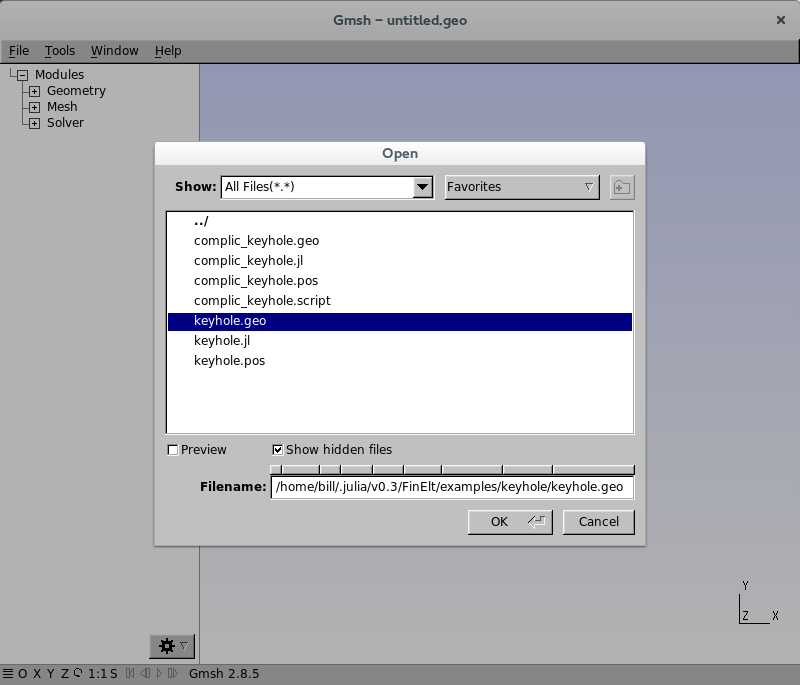
\includegraphics[scale=0.4]{images/open_geo_file.png}
\end{center}
\end{figure}

\begin{figure}
\caption{The Gmsh options window.}
\label{fig: options}
\begin{center}
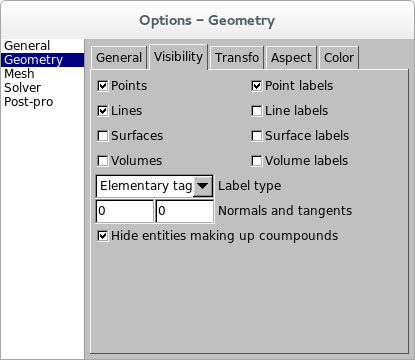
\includegraphics[scale=0.4]{images/options.png}
\end{center}
\end{figure}

\begin{figure}
\caption{A triangulation of $\Omega$.}
\label{fig: triangulation}
\begin{center}
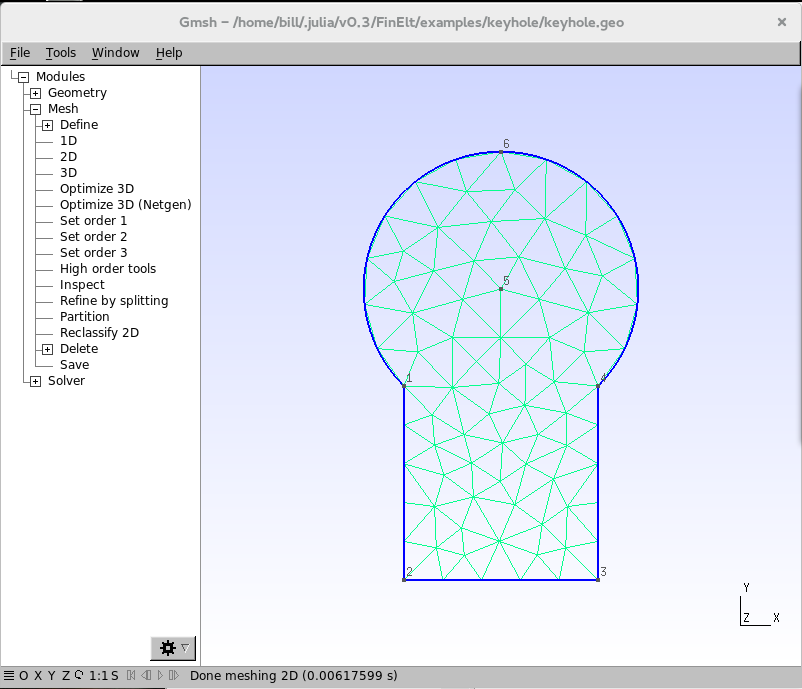
\includegraphics[scale=0.4]{images/triangulation.png}
\end{center}
\end{figure}
%%%%%%%%%%%%%%%%%%%%%%%%%%%%%%%%%%%%%%%%%%%%%%%%%%%%%%%%%%%%%%%%%%%%%%

To compute a numerical approximation to this weak solution, we start 
by triangulating $\Omega$.  Use a text editor to read the 
geometry description file~\verb!keyhole.geo! and observe how the 
domain~$\Omega$ is defined by first specifying the coordinates of 
points around its boundary, and then specifying how these points are 
connected by line segments or circular arcs whose union is~$\Gamma$.  
Notice that Gmsh thinks of $\Omega$ as a surface in 3D (lying in the 
plane~$z=0$).

Start Gmsh and use the \verb!File! menu to open 
\verb!keyhole.geo! as shown in Figure~\ref{fig: open file}.  
From the \verb!Tools! menu, open the \verb!Options! window, select 
\verb!Geometry! in its left pane, and tick the checkbox to display 
\verb!Point labels!; see Figure~\ref{fig: options}.  The main Gmsh 
window should now display the keyhole domain~$\Omega$ and show the 
locations of the points defined in \verb!keyhole.geo!.

To generate a triangulation, click on the \verb!+! next to 
the \verb!Mesh! label in the left pane of the main Gmsh window and 
then click on \verb!2D!.  The result should look something like 
Figure~\ref{fig: triangulation}.  From the \verb!File! menu, select 
the \verb!Save Mesh! option to create a text file 
\verb!keyhole.msh!.

Let $\Omega_h$ denote the triangulated domain, where, in the customary
way, $h$ is the maximum diameter of the triangles.  Since $\Omega_h$ 
is a polygon it can only approximate $\Omega$, whose boundary 
$\Gamma$ contains circular arcs.  We introduce the finite element 
space~$\mathcal{S}_h$ made up of the functions 
$v:\Omega_h\to\mathbb{R}$ that are continuous, piecewise-linear and 
vanish on~$\partial\Omega_h$.  The finite element 
solution~$u_h\in\mathcal{S}_h$ is then defined by requiring that
\begin{equation}\label{eq: finite elt problem}
\int_{\Omega_h}\nabla u_h\cdot\nabla v=\int_{\Omega_h} 4v
	\quad\text{for all $v\in\mathcal{S}_h$,}
\end{equation}
which is a finite-dimensional approximation to the variational 
problem~\eqref{eq: weak bvp}.

Use a text editor to read the file \verb!keyhole.jl!.  This 
Julia script begins by reading the mesh data file \verb!keyhole.msh! 
and creating a data structure called \verb!mesh! that stores (amongst 
other things) the coordinates of the vertices of the triangulation as 
well as the connectivity matrix that specifies which points make up 
each triangle.  Look in the file
\verb!FinElt/Gmsh.jl! to see how this data structure is defined via 
the \verb!Mesh! type.  

The script then creates a second data structure~\verb!vp! that 
describes the variational problem; look in \verb!FinElt/FEM.jl!.  We 
specify that an essential (that is, Dirichlet) boundary condition 
applies over all of~$\Gamma$.  (Zero boundary values are assumed by 
default.)  Next, we specify the bilinear form on the LHS 
of~\eqref{eq: finite elt problem}, and the linear functional on the 
RHS.

Once \verb!vp! is completely specified, the script generates the 
(sparse) linear system for the degrees of freedom, that is, the 
values of~$u_h$ at the interior nodes of the triangulation.  This 
linear system is solved using the \verb!\! operator and the full 
nodal vector~\verb!u! is constructed by including the values at both 
the free and fixed nodes (the latter being all zeros).  As output, 
the script writes a postprocessing file \verb!keyhole.pos!.

Execute the script in the usual way:
\begin{verbatim}
julia> include("keyhole.jl")
\end{verbatim}
To visualize the solution, return to the Gmsh main window.  From 
the \verb!File! menu, select \verb!Merge! and choose 
\verb!keyhole.pos!; the result should look like 
Figure~\ref{fig: postprocess}.  You might encounter a bug in Gmsh 
that corrupts the display.  If so, select \verb!Clear! from the 
\verb!File! menu, then use \verb!Open! (or \verb!Open recent!) to 
reload \verb!keyhole.msh!, and finally \verb!Merge! to read 
\verb!keyhole.pose!.

%%%%%%%%%%%%%%%%%%%%%%%%%%%%%%%%%%%%%%%%%%%%%%%%%%%%%%%%%%%%%%%%%%%%%%
\begin{figure}
\caption{View after merging the postprocessing file.}
\label{fig: postprocess}
\begin{center}
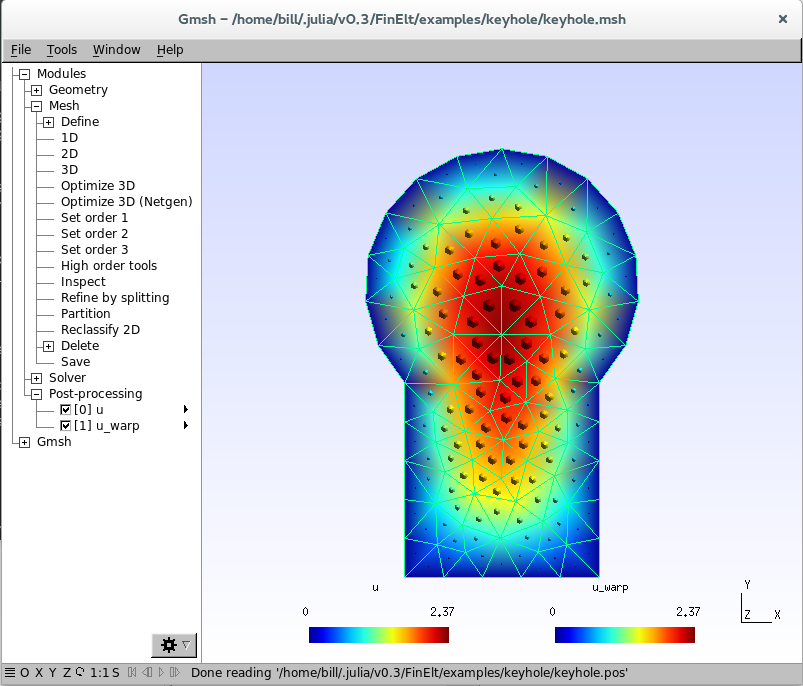
\includegraphics[scale=0.4]{images/postprocess.png}
\end{center}
\end{figure}

\begin{figure}
\caption{The Warp plugin.}
\label{fig: Warp}
\begin{center}
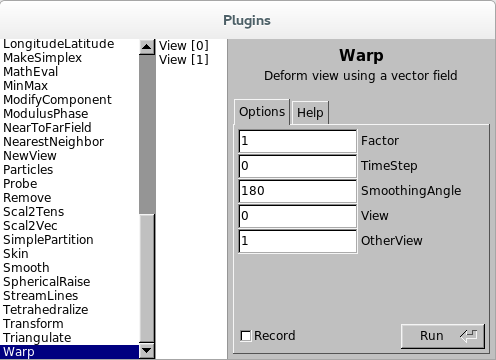
\includegraphics[scale=0.4]{images/warp.png}
\end{center}
\end{figure}

\begin{figure}
\caption{View after warping the surface.}
\label{fig: warped surface}
\begin{center}
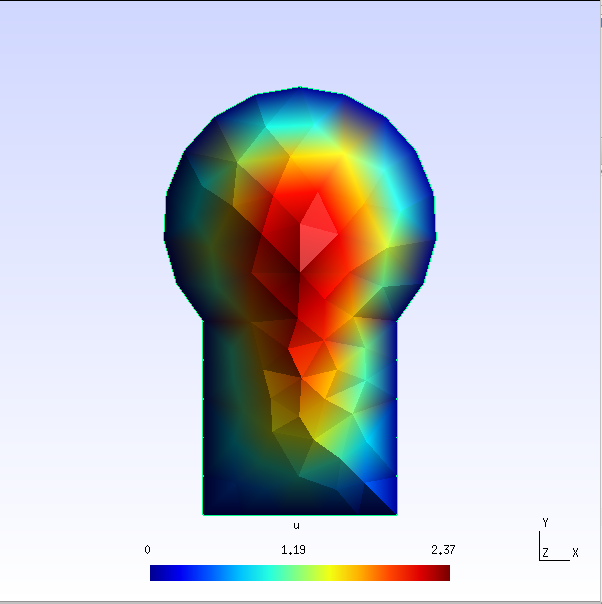
\includegraphics[scale=0.4]{images/warped_surface.png}
\end{center}
\end{figure}

\begin{figure}
\caption{View after using the mouse to rotate the surface in 3D.}
\label{fig: 3D view}
\begin{center}
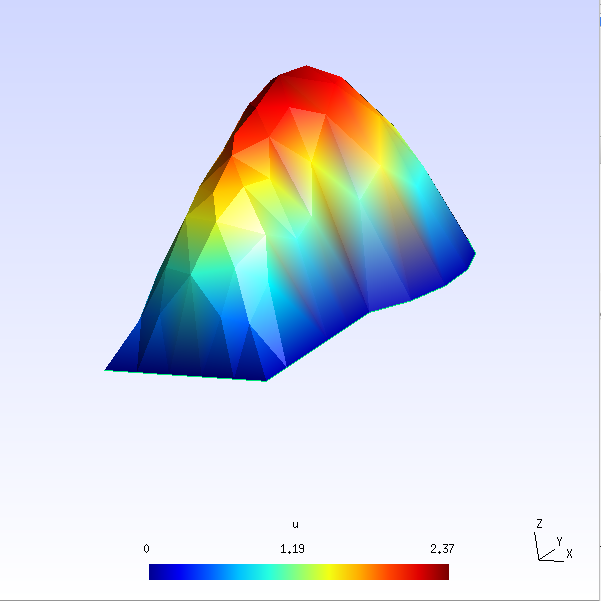
\includegraphics[scale=0.4]{images/3Dview.png}
\end{center}
\end{figure}
%%%%%%%%%%%%%%%%%%%%%%%%%%%%%%%%%%%%%%%%%%%%%%%%%%%%%%%%%%%%%%%%%%%%%%

In the left pane of the Gmsh window, under \verb!Post-processing!, 
are two check boxes labelled \verb!u!~and \verb!u_warp!.
Uncheck the second of these; the display should now look more 
reasonable.  However, because Gmsh is really a 3D mesh generator, 
when solving a 2D problem we have to use something 
of a kludge to obtain a surface plot of the solution.  From the 
\verb!Tools! menu, open the \verb!Plugins! window,  
scroll to the bottom of its left pane and select \verb!Warp!.  In the 
right pane, change \verb!View! from \verb!-1! to \verb!0!, and change 
\verb!OtherView! from~\verb!-1! to~\verb!1!; see Figure~\ref{fig: 
Warp}.  After clicking the \verb!Run! button, you should see something 
like Figure~\ref{fig: warped surface}.  By left-clicking and dragging 
the display, you can rotate the surface to obtain a view like the one 
in Figure~\ref{fig: 3D view}.

%%%%%%%%%%%%%%%%%%%%%%%%%%%%%%%%%%%%%%%%%%%%%%%%%%%%%%%%%%%%%%%%%%%%%%
\section*{Second Example}
%%%%%%%%%%%%%%%%%%%%%%%%%%%%%%%%%%%%%%%%%%%%%%%%%%%%%%%%%%%%%%%%%%%%%%
\begin{thebibliography}{0}
\bibitem{Gmsh}
C.~Geuzaine and J.-F.~Remacle. Gmsh: a three-dimensional finite 
element mesh generator with built-in pre- and post-processing 
facilities. \emph{International Journal for Numerical Methods in 
Engineering} 79(11), pp.~1309--1331, 2009.
\end{thebibliography}
%%%%%%%%%%%%%%%%%%%%%%%%%%%%%%%%%%%%%%%%%%%%%%%%%%%%%%%%%%%%%%%%%%%%%%
\end{document}
